\chapter{Verktyg som är lämpliga för att skriva stora dokument}
\label{cha:indiv-report-tuhkala}
\chapterprecis{\LARGE{---- Hannes Tuhkala ----}}

\section{Inledning}
\label{sec:introduction-tuhkala}
Att skapa bra och stiliga dokument är viktigt för att det ska se professionellt ut. I den här rapporten kommer en undersökning som är gjord av Hannes Tuhkala om vilka fördelar och nackdelar som \latex och Word har för att skriva stora dokument. Rapporten tar också upp vilka verktyg som lämpar sig för att skriva stora dokument.

\subsection{Syfte}
\label{sec:purpose-tuhkala}
Syftet med den här rapporten är att ta reda på vilka för- respektive nackdelar som finns med att använda \latex och Word för att framställa dokument. Syftet är också att undersöka vilka asynkrona eller synkrona verktyg som är lämpliga att använda för att skriva stora dokument samt vilka erfarenheter projektgruppen kan ta med sig ifrån projektet gällande dokumenthantering.

\subsection{Frågeställning}
\label{sec:issue-tuhkala}
De frågeställningar som rapporten behandlar är:

\begin{enumerate}
	\item Vilka fördelar och nackdelar finns det med att använda \latex eller Word när man skriver dokument?
	\item Vilka verktyg lämpar sig för att skriva större dokument?
	\item Vilka erfarenheter kan tas med ifrån det här projektet gällande framställning av större dokument?
\end{enumerate}

\subsection{Definitioner, akronym och förkortningar}
Följande definitioner och förkortningar används på flertalet ställen i den här rapporten:

\begin{itemize}
	\item Ett större dokument - Definierar här som ett dokument som två eller flera personer arbetar på och är åtminstone sju sidor långt.
	\item Synkront verktyg - Ett program eller en tjänst som flera personer kan skriva samtidigt på utan att man behöver vänta på att någon annan skrivit färdigt.
	\item Asynkront verktyg - Ett program eller en tjänst som en person skriver text på och skickar det till andra personer efteråt.
	\item SVN - Apache Subversion
	\item Word - Microsoft Word
	\item WYSIWYG editor - WYSIWYG editor står för (What You See Is What You Get) editor och är ett program eller system där innehåll kan ändras på ett sätt sådant att det liknar hur det slutgiltiga dokumentet kommer att se ut.
	\item Separata filer - Se avsnitt \ref{sec:thesis-info-tuhkala}.
	\item Gemensam fil - Se avsnitt \ref{sec:thesis-info-tuhkala}.
\end{itemize}

\subsection{Avgränsningar}
Denna rapport kommer endast att ta upp de två vanligaste typsättningssystemen, \latex och Microsoft Word eftersom de är de mest använda och kända. Det finns liknande system som dessa, till exempel OpenOffice eller LibreOffice och de kommer inte att behandlas i rapporten för att de inte är lika välanvända och kända. Rapporten kommer också att ta upp olika asynkrona verktyg som Git, SVN och Mercurial samt synkrona verktyg som Google Docs, ShareLaTeX och Overleaf. Dessa valdes också för att de är de vanligaste tjänsterna och mest använda.

\section{Bakgrund}
\label{sec:background-tuhkala}
Vi har arbetat med olika verktyg för att framställa större dokument för projektet i gruppen. Vi har använt oss av LaTeX för alla våra större dokument och använt oss av både asynkrona och synkrona verktyg när vi skrev dessa. För alla större dokument utom kandidatrapporten användes ett synkront verktyg, Overleaf. För kandidatrapporten använde vi oss av ett asynkront verktyg, Git. Den här studien har genomförts för att se vilket av de olika asynkrona och synkrona verktygen som kan vara bättre att använda sig utav för större dokument. Flera andra verktyg har också tagits upp för att se hur andra projektgrupper framställer sina dokument. 

\section{Teori}
\label{sec:theory-tuhkala}
Nedan visas information om det som kommer att tas upp i rapporten. Det ger lite teori om vad \latex, Git och SVN är för något.

\subsection{\latex}
\latex är ett typsättningssystem som är baserat på TeX och skapades för att göra det enklare att skapa generella böcker och artiklar inom TeX. Till skillnad från till exempel Microsoft Word, programmerar man dokumentet, istället för att skriva formaterad text. \latex bygger på att den som skriver inte ska formatera texten, utan ska bara skriva det den vill få sagd, utan att behöva bry sig om hur dokumentet ser ut. Det är därför väldigt enkelt att få stiliga dokument i \latex genom att bara specifiera dokumentets struktur istället för att krångla med hur dokumentet ska se ut.

\subsection{Git}
Git är ett versionshanteringsprogram som skapades av Linus Torvalds för att hantera källkoden till Linuxkärnan. Git är ett så kallat distribuerat versionshanteringssystem, vilket innebär att alla som använder ett Git repository har allt som det innehåller och behöver inte använda en centraliserad server. Git har också komplett historik över alla ändringar som skett och man kan gå tillbaka till tidigare versioner av dokument och källkod.

\subsection{Apache Subversion}
Subversion (SVN) är också ett versionshanteringsprogram för mjukvara likt Git, förutom att SVN är ett centraliserat versionshanteringssystem.

\subsection{Mercurial}


\subsection{Kandidatrapport}
\label{sec:thesis-info-tuhkala}
Kandidatrapporten är skriven i \latex och använder mallen för avhandlingar skapad av Ola Leifler \cite{thesis_template}. Mallen är upplagd så att det finns separata filer för varje del av rapporten istället för en enstaka stor fil. Det innebär att introduktion, bakgrund, metod, de individuella bidragen samt de andra delarna i rapporten är separata filer.

\section{Metod}
\label{sec:method-tuhkala}
För att kunna besvara frågeställningarna har jag delat upp dem i tre sektioner för hur jag gick tillväga för att svara på dem.

\subsection{Första frågeställningen}
För min första frågeställning gjordes en litteraturstudie för att samla information om vilka för- och nackdelar som finns med att använda \latex eller Word när man skriver dokument. Detta för att se hur tidigare arbeten ställer sig till sde två olika typsättningssystemen som jag tar upp i frågeställningen.

\subsection{Andra frågeställningen}
För min andra frågeställning gjordes en enkätundersökning som skickades ut till alla som läser kursen TDDD96, Kandidatprojekt i programvaruutveckling. I enkäten ställdes först dessa frågor:
\begin{itemize}
	\item Vilken grupp är du i?
	\item Vilket verktyg använder ni när ni skriver de flesta större/viktiga dokument?
\end{itemize}
Beroende på hur de svarade på föregående fråga "Vilket verktyg använder ni när ni skriver de flesta större/viktiga dokument?" får de olika frågor. Om de valde alternativ 1 (Asynkrona verktyg som Git, SVN och liknande) fick de följande frågor:
\begin{itemize}
	\item Vad för slags versionshanterare använder ni er av?
	\item Hur nöjd är du med hur ni versionshanterar era dokument?
	\item Om du fick ändra vilket asynkront versionshanteringsverktyg ni använde, vilket hade du då valt?
	\item Skulle du vilja byta hantering av dokument till synkrona verktyg som Google Docs, ShareLaTeX och liknande?
	\item Om du svarade ja, vilket verktyg skulle du då vilja använda?
\end{itemize}
Om de valde alternativ 2 (Synkrona verktyg som Google Docs, ShareLaTeX och liknande) fick de besvara dessa frågor istället:
\begin{itemize}
	\item Vilken webbsida/tjänst använder ni er av för större/viktiga dokument?
	\item Hur nöjd är du med att använda en tjänst som denna för hantering av dokument?
	\item Om du fick byta den tjänst ni använde, vilken hade du då valt?
	\item Skulle du vilja byta hantering av dokument till asynkrona verktyg som Git och SVN?
	\item Om du svarade ja, vilket verktyg skulle du då vilja använda?
\end{itemize}
Till sist frågades också detta oberoende av vilka alternativ man valt.
\begin{itemize}
	\item Vilka verktyg som har listats här tycker du är bra för större dokument?
\end{itemize}

\subsection{Tredje frågeställningen}

För min tredje frågeställning gjordes också en enkätundersökning men enbart för medlemmarna i projektgruppen. Där ställdes dessa frågor:
\begin{itemize}
	\item Överlag hur tycker du att hanteringen av större dokument har gått i gruppen?
	\item Vilket verktyg tycker du har varit bäst att använda?
	\item Varför tycker du det?
	\item För kandidatrapporten, tycker du att det var bättre med separata filer än en gemensam fil?
\end{itemize}

\section{Resultat}
\label{sec:results-tuhkala}
Resultatet som jag kommit fram till från min litteraturstudie och de två enkäter som beskrevs i metoden visas nedan.

\subsection{Litteraturstudie}
Knauff och Nejasmic \cite{knauff2014efficiency} visar med hjälp av ett mjukvaruanvändbarhetstest hur effektivt det är att använda sig av \latex jämfört med Microsoft Word. Testet gick ut på att 40 deltagare över olika vetenskapsgrenar skulle skriva olika vetenskapliga texter.
Det visar sig att \latex användare var långsammare än Word användare, skrev mindre text på samma tid och gjorde fler grammatiska-, formatterings- och typsättningsfel. På de flesta tester var experter i \latex sämre än nybörjare i Word. \latex användare säger sig tycka om att använda det än andra typsättningssystem. Författarna kom till slutsatsen att erfarna \latex användare kan drabbas av produktivitetsförlusta än andra typsättningssystem.

Loch et al. \cite{loch2014master} tar upp om Word är ett lämpligt verktyg för studenter att typsätta matematik istället för \latex. Den artikeln tar också upp hur Word jämför sig med andra matematiska typsättningspaket som studenter har använt. De kommer fram till att nuvarande versioner av Word är kapabla att skapa matematiska texter med hög kvalitet. De säger också att inlärningskurvan inte är väldigt hög och att Word inte ska avfärdas för matematiska texter.  

Henrik Henrikssons bidrag i Haavisto et al. \cite{Haavisto954095} tittar på vilka problem som nybörjare i \latex stöter på och hur man kan förhindra sådana problem i framtida projekt. Han kommer fram till att det är mycket konsistensproblem i ett \latex dokument. Många skriver text olika och det finns ingen standard. Förslag på hur man kan lösa problemen är att använda en linter eller sätta upp en standard i början av projektet.

\subsection{Enkät 1}
Resultaten från den första enkäten, enkäten om hur det är att använda sig av synkrona respektive asynkrona verktyg när man skriver stora dokument visas nedan. Om mer detaljerade resultat önskas, se Bilaga \ref{appendix:svar_enkat_dokument}.\\
Totalt sett var det 36 av 98 personer som svarade på enkäten. Det ger ett deltagande på 36,7\%.\\
\\\textbf{Vilket verktyg använder ni när ni skriver de flesta större/viktiga dokument?}\\
En tredjedel av grupperna använder sig av ett asynkront verktyg, alltså Git, SVN och liknande. Resterande grupper använder sig av ett synkront verktyg som ShareLaTeX, Google Docs och liknande.\\\\
De som valde alternativ 1 (Asynkrona verktyg som Git, SVN och liknande) visas nedan. Totalt sett var det en tredjedel av grupperna som använde detta varav 15 personer som svarade.\\\\
\textbf{Vad för slags versionshanterare använder ni er av?}\\
Alla grupper som använder sig av ett asynkront verktyg använder sig av Git.\\\\
\textbf{Hur nöjd är du med hur ni versionshanterar era dokument?}\\
Från en skala från 1 till 5 där 1 är inte nöjd och 5 är nöjd, är medelvärdet 4.466 ~= 4.5.\\\\
\textbf{Om du fick ändra vilket asynkront versionshanteringsverktyg ni använde, vilket hade du då valt?}\\
Ingen av deltagarna vill byta det asynkrona verktyg de använder till ett annat, utan de vill fortsätta använda Git.\\\\
\textbf{Skulle du vilja byta hantering av dokument till synkrona verktyg som Google Docs, ShareLaTeX och liknande?}\\
40\% av deltagarna vill byta till ett synkront verktyg istället för det asynkrona verktyg de använder nu. 60\% vill fortfarande använda sig av Git.\\\\
\textbf{Om du svarade ja, vilket verktyg skulle du då vilja använda?}\\
Av de som vill byta till synkront verktyg skulle två tredjedelar vilja byta till ShareLaTeX och en tredjedel byta till Google Docs.\\\\
De som valde alternativ 2 (Synkrona verktyg som Google Docs, ShareLaTeX och liknande) visas nedan. Totalt sett var det två tredjedelar av grupperna som använde detta varav 21 personer som svarade.\\\\
\textbf{Vilken webbsida/tjänst använder ni er av för större/viktiga dokument?}\\
3 av grupperna som använder ett synkront verktyg använder ShareLaTeX. Lika många grupper använder sig istället av Overleaf. En grupp använder sig av Google Docs och en annan grupp använder sig av Office 365 Word.\\\\
\textbf{Hur nöjd är du med att använda en tjänst som denna för hantering av dokument?}\\
Från en skala från 1 till 5 där 1 är inte nöjd och fem är nöjd, är medelvärdet på hur nöjda de är 3.8.\\\\
\textbf{Om du fick byta den tjänst ni använde, vilken hade du då valt?}\\ 
13 av de som fick frågan ville inte byta den synkrona tjänsten som de använde. Två vill använda sig av Google Docs istället. En person vardera ville byta tjänst till Overleaf och ShareLaTeX. En annan ville ha en kombination av en "online-tjänst" och Git. Två vill byta till \latex och Git.\\\\
\textbf{Skulle du vilja byta hantering av dokument till asynkrona verktyg som Git och SVN?}\\
15 deltagare vill inte byta till ett asynkront verktyg medan sex personer ville byta verktyg.\\\\
\textbf{Om du svarade ja, vilket verktyg skulle du då vilja använda?}
De som ville byta till ett asynkront verktyg vill använda sig av Git istället.\\\\
Den sista frågan som ställdes till alla deltagare i undersökningen oberoende av vad de tidigare valt:\\\\
\textbf{Vilka verktyg som har listats här tycker du är bra för större dokument?}\\
Figur \ref{fig:best_document_tool} visar svaret för frågan. På x-led finns de olika alternativen man kunde välja och y-led visar hur många som valt det alternativet. Från figuren ser man att Git, Google Docs och ShareLaTeX är det verktyg de flesta valt.

\begin{figure}[H]
	\centering
	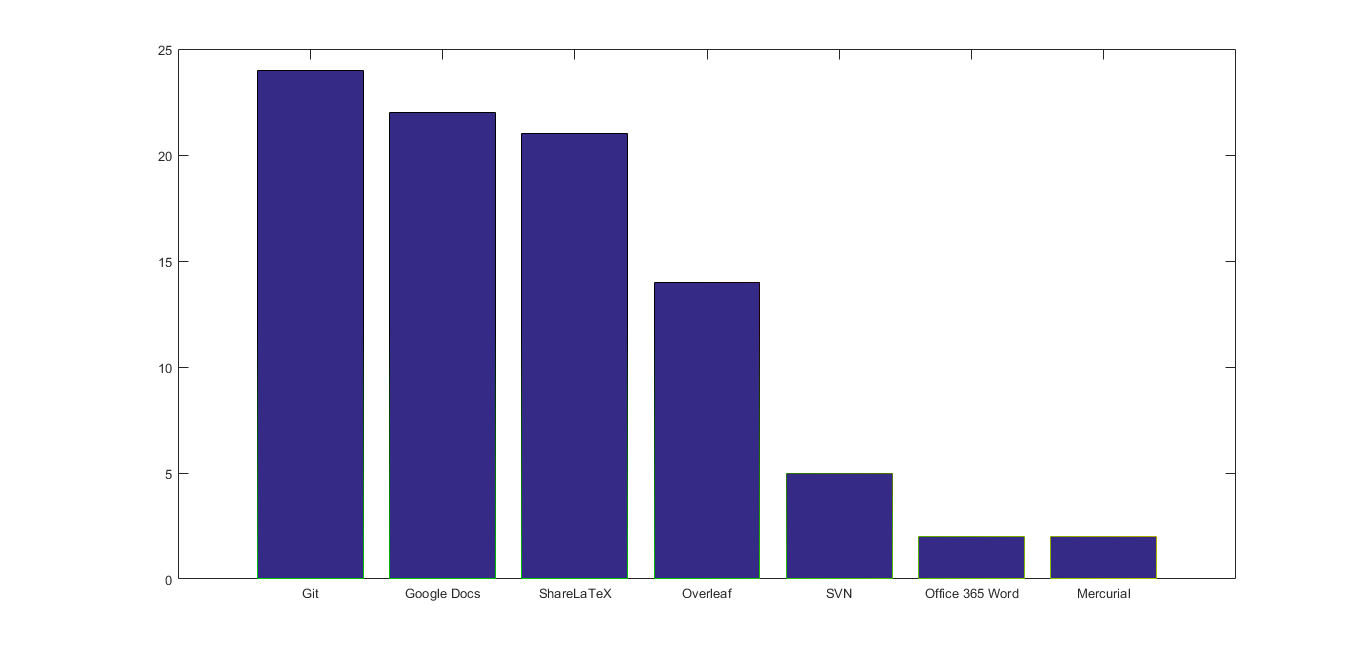
\includegraphics[width=150mm,height=75mm]{figures/best_document_tool.png}
	\caption{Visar resultatet från vilka verktyg som deltagarna tycker är bra för större dokument.}
	\label{fig:best_document_tool}
\end{figure}

\subsection{Enkät 2}
Resultaten från den andra enkäten, den om vilka erfarenheter gruppen kan ta ifrån det här projektet visas nedan. Om mer detaljerade resultat önskas, se Bilaga \ref{appendix:svar_enkat_dokument_erfarenheter}. Totalt var det 6 personer som svarade på enkäten.\\
\textbf{Överlag hur tycker du att hanteringen av större dokument har gått i gruppen?}\\
Fem av sex personer tycker att hanteringen av större dokument har gått bra, och en av dem tycker att det gått väldigt bra. En person tycker att det gått helt okej men kunde varit bättre.\\\\
\textbf{Vilket verktyg tycker du har varit bäst att använda?}\\
En person har ingen åsikt på frågan och en annan person tycker att båda verktygen varit lika bra att använda för större dokument. Fyra personer tycker att kombinationen \latex och Git var det bästa att använda.\\\\
\textbf{Varför tycker du det?}\\
Personen som inte har någon åsikt i frågan och den som tyckte att båda alternativen var bra, tycker inga av alternativen har varit bäst, båda verktygen hade sina egna problem. \latex och Git fungerade smidigare, hade versionshantering, historik och vem som skrivit vad, är de bra delarna av de som tyckte att \latex och Git var bättre att använda.\\\\
\textbf{För kandidatrapporten, tycker du att det var bättre med separata filer än en gemensam fil?}\\
Alla deltagare i enkäten tyckte att separata filer var bättre att använda än en stor gemensam fil för kandidatrapporten.

\section{Diskussion}
\label{sec:discussion-tuhkala}
Nedan kommer min diskussion om resultaten jag fått. De är indelade efter frågeställningarna.

\subsection{Vilka fördelar och nackdelar finns det med att använda \latex eller Word när man skriver dokument?}
Att LaTeX användare var långsammare att skriva än Word användare tycker jag inte är jättemärkligt, eftersom att de som använder LaTeX skriver mer än de som skriver Word. Detta för att LaTeX användarna måste skriva kommandon för att åstadkomma en viss sak medan Word användare behöver bara använda sig av WYSIWYG-editor som finns inbyggd i Word där man klickar på knappar och drar tabeller i dokumentet. Word användare använder också ett anpassat program för att skriva dokument, likt en IDE för programmering. LaTeX har inte lika många anpassade editorer som Word, utan där kompilerar man dokumenten istället och skriver texten i någon annan editor som vanligtvis inte har stöd för LaTeX kommandon.

Från resultatet ser vi också att inlärningskurvan för Word inte är väldigt stor och kräver inte mycket av en för att förstå och använda programmet. Det håller jag med om eftersom man behöver inte lära sig kommandon, hur man kompilerar och hur man sätter upp sin \latex-miljö. I Word får man ett program som är en WYSIWYG-editor, där man för det mesta skriver texten man vill få fram.

Det Henrik Henriksson tog upp i sin rapport om att ha en standardisering på \latex dokument skulle ha gjort att våra dokument såg likadant ut överallt. Det hade varit bättre, för till exempel när vi använde Overleaf var det några som använda mellanslag för indentering och andra som använde tabbar för det. För en del av medlemmarna i gruppen var det första gången de använda \latex och det hade kunnat vara lättare för dem om man hade en standardisering och instruktioner för hur \latex fungerar. Att använda en linter hade också hjälpt att hitta fel i dokumentet fortare än att behöva kompilera och få kompileringsfel. Overleaf hade ingen linter vilket hade gjort det svårt att införa det där men det finns som sagt alternativ till det.

\subsection{Vilka verktyg lämpar sig för att skriva större dokument?}
Att alla grupper som använder sig av asynkrona verktyg använder Git förvånar mig inte, just eftersom det är ett bra verktyg för att versionshantera dokument och källkod bland annat. Jag förväntade mig dock att någon grupp använde SVN eller Mercurial. De som använt sig av Git har varit väldigt nöjda och gett ett medelvärde på 4.5 på en skala från 1 till 5 på hur nöjda de varit tycker jag låter rimligt, för att det är ett väldigt bra verktyg. Eftersom jag tog ett par snarlika alternativ som till exempel Git, SVN och Mercurial samt ShareLaTeX och Overleaf där funktionaliteten inte skiljer sig så mycket åt kanske det hade varit bättre att bara fråga mer generellt om asynkrona verktyg är bättre att använda än synkrona verktyg.

För synkrona verktyg skiljer medelvärdet med 0.7 till 3.8 än för 4.5 för asynkrona. Det är också väldigt bra och jag tycker också det är bra att kunna ändra på dokument samtidigt i Overleaf och Google Docs. Majoriteten vill inte byta synkron verktyg eller byta till ett asynkront. Det tror jag kan bero på att de inte testat att använda sig av ett asynkront verktyg.

På den sista frågan i resultatet finns det flera alternativ som ligger i topp: Git, Google Docs, ShareLaTeX och Overleaf. Ett av dem är asynkront och resten är synkrona. Jag har själv använt alla förutom ShareLaTeX fast jag tror inte det skiljer sig mycket med Overleaf, och jag tycker att alla är väldigt bra att använda för att skapa stora dokument. Om det fanns ett verktyg som kunde kombinera versionshantering med att skriva samtidigt i samma dokument tror jag det skulle ha varit bättre att använda. Detta för att man får allt i båda världar: Versionshantering och historik samt att kunna skriva samtidigt. Hur det skulle fungera vet jag dock inte.

En del av alternativen jag hade till frågorna hade inte valts alls, och jag hade inget som frågade varför man inte valde dem. Det kan ju ha varit för att man inte visste vad verktyget var för något, till exempel för Mercurial. Det kan också vara för att de inte visste vad skillnaden var mellan verktygen, om man till exempel bara använt ett av dem. Det kan också ha varit för att de inte tyckt att det var något bra alternativ alls. Det är svårt att veta utan att ha frågat om det. 

\subsection{Vilka erfarenheter kan tas med ifrån det här projektet gällande framställning av större dokument?}
Att majoriteten tycker att sättet vi arbetade med kandidatrapporten jämfört med de andra stora dokument är bättre håller jag med om. Det var enklare att ha versionshantering och historik, för att man kunde se vad som ändrades eller lades till vid varje version och vem som utförde det. Man kan gå tillbaka till en tidigare version med ett enkelt kommando. Detta kunde vi inte göra när vi använde Overleaf. Fördelen med det var att alla kunde skriva samtidigt och man inte behövde installera någon mjukvara för det. Det jag tycker var mindre bra med Git och \latex var att stycken oftast skrevs som en rad vilket ger många konflikter när man försöker sammanfoga varandras delar om man ändrat något, stort eller litet.

\subsection{Metod}
Litteraturstudien för frågeställning 1 kunde kanske ha gett ett annat eller mer utförligare svar om fler artiklar, bloggar och liknande hittats. Nu när det är rätt så få källor som jag hittat kan det ge en missrepresentativ bild av det.

Enkätundersökningen som gjordes för den andra frågeställningen kunde ha gjorts mer utförligare, genom att ställa bättre frågor eller fråga om mer utförligare svar. Till exempel "Rangordna de olika alternativen från det du hade helst använt till det du helst inte velat använda." istället för att endast bara fråga om "Vilka alternativ hade du använt i framtiden för större dokument?". Om fler personer hade svarat på den första enkäten kunde det ha gett en bättre bild på hur det ser ut. Om man låtit deltagarna testat de olika verktygen innan enkäten hade det nog gett ett bättre resultat. Jag tror inte att de flesta som gjorde enkäten testat alla alternativ utan möjligtvis två stycken.

Urvalsgruppen är alla projektgrupper som läser kandidatprojektet och det kanske inte ger en representativ generell bild av arbete på större dokument än om urvalsgruppen innehållit andra yrken eller liknande. Vissa av alternativen kan förekomma mer inom företag än andra ställen.

Den andra enkätundersökningen kunde ha haft en till fråga "Vad var det som var dåligt med hanteringen av större dokument?". Som det ser ut nu får man bara de bra sakerna med verktygen. Kunde också ha frågat om det finns något annat verktyg än de vi använde som kunde ha varit bättre. Att använda sig av en enkät för att ta reda på vad gruppmedlemmar tycker kan både vara bra och dåligt. Det dåliga är att det bara är mina frågor som kommer fram medan andra frågor kan komma upp om man intervjuar istället. Det blir lite skillnad på en enkät och en intervju. Det som är bra är att det går fort att göra och att det är enklare att sammanställa svaren.

\subsection{Källkritik}

\section{Slutsatser}
\label{sec:conclusions-tuhkala}
Nedan visas slutsatserna som kommit fram från resultatet för de tre frågeställningarna:

\subsection{Vilka fördelar och nackdelar finns det med att använda \latex eller Word när man skriver dokument?}
Det jag fått fram genom min litteraturstudie är att båda alternativen har fördelar och nackdelar samt att det inte skiljer sig mycket mellan dem. Word användare skriver dokument snabbare än vad \latex användare gör. Inlärningskurvan är inte särskilt stor för att lära sig och använda Word. För att skriva större matematiska texter är det ingen skillnad mellan alternativen eftersom båda gör det med hög kvalitet. Att ha en standardisering och utbildning i \latex kan hjälpa nybörjare.

\subsection{Vilka verktyg lämpar sig för att skriva större dokument?}
Det jag kommit fram till med hjälp av min enkätundersökning är att Git, Google Docs och ShareLaTeX kan vara bra verktyg att använda sig av när man skriver större dokument. Overleaf kan också vara ett bra verktyg att använda sig av. Mindre lämpliga verktyg att använda är SVN, Office 365 Word och Mercurial. De verktyg som dem använde i gruppen är de väldigt nöjda med.

\subsection{Vilka erfarenheter kan tas med ifrån det här projektet gällande framställning av större dokument?}
De erfarenheter som kan tas med ifrån detta projekt är att \latex och Git har varit det bästa verktyget att använda vid framställning av större dokument. \latex och Overleaf har också varit bra men fördelarna med Git har övervägt det. Separation av dokumentet i flera mindre filer har också varit bättre än att ha en stor gemensam fil.

%%%%%%%%%%%%%%%%%%%%%%%%%%%%%%%%%%%%%%%%%%%%%%%%%%%%%%%%%%%%%%%%%%%%%%
%%% tuhkala-report.tex ends here
